\section{Modeling Restore Effects}
Modeling and simulation are required to perform the studies on further scaling DRAM. On device level, the model needs to capture the critical components including transistor, capacitor, sense amplifier, and other peripheral circuits; and the model should also cover the primary parameters and dimensions, such as transistor length/width, capacitance and voltage, etc. Following the principles, we built SPICE modeling on basis of a Rambus tool \cite{MICRO10:rambus}, and simulated data write operation. %The simulation is repeatedly performed on 20nm and 14nm technology nodes.


Further, to involve process variation effects, the models should be inherently statistical following certain distributions.
Using the aforementioned cell model, we generate 100K samples and curve fit using log-normal distribution. Similar to recent PV studies \cite{ISCA12:raidr,HPCA14:mosaic}, we include bulk distribution to depict the normal variation that dominates the majority of cells, and tail distribution to depict random manufacturing defects
{\footnote{Note that not all cells following the tail distribution are treated as defects. The worst ones are covered by conventional redundant repairs \cite{HPCA14:mosaic}.}}.
Table \ref{tab:tech} summarizes the parameters for bulk and tail distributions after curve fitting with our cell samples. 

\begin{savenotes}
\begin{table}[htbp]
\vspace{-0.2in}
\caption{Modeling Parameters}
\vspace{-0.2in}
\centering
\scalebox{0.85}
{
\begin{tabular}{l|llll|lcc}
\hline
tech node&	$\mu_{bulk}$&	$\sigma_{bulk}$&	$\mu_{tail}$&	$\sigma_{tail}$&	$\phi$&	random weight\\
\hline\hline
%20nm&	2.031&	0.21&	3.081&	0.063&		0.3	&0.5\\
14nm \footnote{Whereas we modeled both 20nm and 14nm nodes, here we only show the case of 14nm because of space limitation. Data and results on 20nm can be found in \cite{DATE15:twr}.} &	2.048&	0.247&	3.283&	0.0735&	0.3	&0.5\\
\hline\hline
\end{tabular}
}
\label{tab:tech}
\end{table}
\end{savenotes}

To obtain the chip maps, we use the VARIUS tool \cite{SM08:varius} to involve both within-die (WID) and die-to-die (D2D) process variations. 
Similar to prior PV studies \cite{ICICDT:weight,HPCA14:mosaic}, we assume the same share of systematic and random components, and choose $\phi=0.3$ meaning that the correlation range equals to 30\% of the chip's side length, as shown in Table \ref{tab:tech}. 
With the constructed models and collected parameters, then we can move forward to generate chips, and then form ranks and DIMMs using the pool of chips. Next, architectural explorations can be conducted on the collected memory system. 
%To get close to real manufacturing process, it is necessary to guarantee the quantities of chips, ranks and DIMMs large enough to be swept over in simulations.

\section{Proposed Designs}
In this section, we elaborate the proposed designs. First, we discuss the post-fabrication schemes in terms of both coarse chip-level and fine chunk-level restoring management; then, we extend the schemes to assembly phase to deliberately form ranks by clustering compatible chips; and finally, the schemes are integrated with OS-level page allocation to maximum performance gains.

\subsection{Chip-specific Restoring Control}
Conventionally, a single set of timing constraints is applied to the whole memory system, which totally ignores the existing variations and thus a too conservative setting.
A simple enhancement can be made by exposing chip variations, i.e., setting different {\tt tWR}s for different chips. 
%For this purpose, a post-fabrication test process is performed by the manufacturer to determine the {\tt tWR} of each chip while a DIMM is then constructed using chips with the same or similar {\tt tWR}s
%\footnote {Differing from later rank formation, here we consider the chip as a whole, which is unaware of the internal distribution.}
%. Each DIMM derives its {\tt tWR} from the chip-row 
%that has the worst {\tt tWR} of the entire DIMM (as shown in Figure \ref{fig:chip_default}), or the worst one after adopting a small number of spares to rescue those slowest chip-rows. 
As illustrated by Figure \ref{fig:chip_default}, the chip-specific {\tt tWR} design helps to improve chip yield rate as otherwise a chip with {\tt tWR}=24ns would be discarded if {\tt tWR} is set as 23ns or less in the standard.  While technically all fabricated chips can now be treated as good ones, those with very large {\tt tWR} (e.g., twice as large as the expected {\tt tWR}) should still be marked as failed chips as DIMMs constructed from them tend to have very low performance. 

\begin{figure}
 \centering
  \begin{subfigure}{.32\textwidth}
    \centering
    	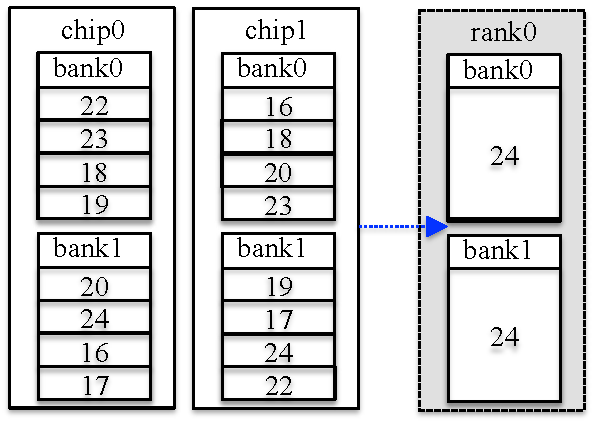
\includegraphics[width=\linewidth]{figures/default.pdf}\\
    \caption{Chip-specific}
    \label{fig:chip_default}
  \end{subfigure}
%
  \begin{subfigure}{.32\textwidth}
    \centering
    	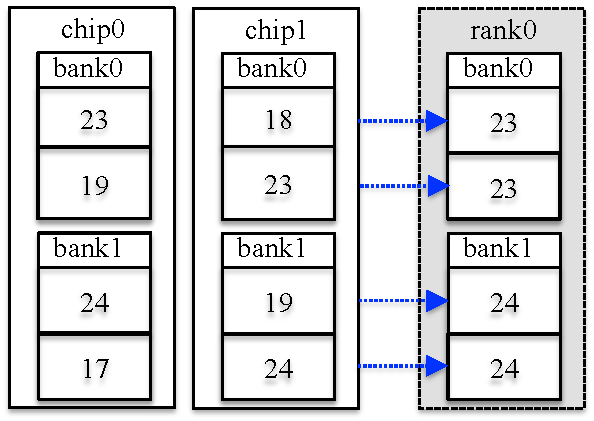
\includegraphics[width=\linewidth]{figures/chunk_unsort.pdf}\\
    \caption{Chunk-specific}
    \label{fig:chunk_unsort}
  \end{subfigure}
  %
  \begin{subfigure}{.32\textwidth}
    \centering
    	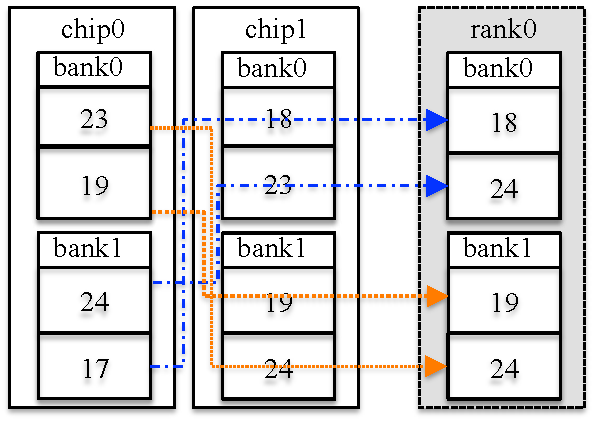
\includegraphics[width=\linewidth]{figures/chunk_sort.pdf}\\
    \caption{Chunk-specific w/ remap}
    \label{fig:chunk_sort}
  \end{subfigure}
  \vspace{-0.45in}
\caption{Comparison of different schemes: (a) The chip-specific {\tt tWR}; (b) The chunk-specific {\tt tWR}; (c) The chunk-specific {\tt tWR} with chunk remapping. For illustration purpose, each rank consists of two chips while each chip contains two four-row banks. One {\underline {\bf DIMM-row}} (i.e., the row exposed to the OS) consists of two {\underline {\bf chip-row}} segments --- the number in each chip-row indicates its corresponding {\tt tWR}, i.e., the {\tt tWR} of the weakest cell.}
\label{fig:schemes}
  \vspace{-0.45in}
\end{figure}

\subsection{Chunk-specific Restoring Control}
Even though {\tt tWR} exhibits a wide range of variations when scaling in deep sub-micron regime, only a small number of cells need long recovery time.  Setting a DIMM's {\tt tWR} based on the chip-row that has the worst {\tt tWR} is still too pessimistic.
We therefore propose to partition each memory bank into a number of smaller chunks and set the chunk level {\tt tWR} based on the worst chip-row within the chunk. 
The chunk level {\tt tWR} is then exposed to the memory controller to aid cheduling.

In Figure \ref{fig:schemes}(b), one chunk consists of two rows. Since the first chunk has 23ns and 18ns {\tt tWR}s for its two chip-rows, its chunk {\tt tWR} is set to 23ns.
By take advantage of these fast chunks, a chunk-{\tt tWR}-aware memory controller can speed up memory accesses that fall into the fast chunks
\footnote{For discussion purpose, a {\em chip-chunk} is referred to as one chunk within one chip; a {\em DIMM-chunk} is referred to as the set of same-index chip-chunks from different chips of the DIMM. For example, the 2nd DIMM-chunk consists of the 2nd chip-chunk from each chip.}.


\subsection{Chunk-specific with Remapping}

The previous design can only form a DIMM-chunk from the same-index chip-chunks, which can be optimized to further reduce {\tt tWR} values. This is because the chip-chunks that are of the same index may exhibit significant {\tt tWR} difference. It would be beneficial to form a chunk using chip-chunks that are of the same or similar {\tt tWR}s. 

For the example in Figure \ref{fig:chunk_sort}, if we form the first DIMM-chunk using the 4th chip-chunk from chip 0 and the 1st chip-chunk from chip 1, the {\tt tWR} of this chunk can be as low as 18ns. Constructing a number of such fast chunks helps to speed up the average row access time of the given DIMM.

The chunk remapping is done in two steps: (1) after detecting the {\tt tWR} for each chip-chunk, we compute the averaged {\tt tWR} for each chip-bank, and sort chip-banks independently on each chip. A {\bf DIMM-bank} consists of chip-banks that are of the same index on the sorted list; (2) For chip-chunks within each chip-bank, we sort them again such that each {\bf DIMM-chunk} consists of chip-chunks that are of the same index on the sorted list. 

While only one access is allowed to access one bank at any time, the multiple banks in a DIMM can be accessed simultaneously. To maintain the same bank level parallelism, we treat the chip-chunks from one bank as a group in chunk remapping. In Figure \ref{fig:schemes}(c), 
DIMM-chunk 0 and 1 belong the DIMM-bank 0. Since DIMM-chunk 0 is constructed using chip-chunk 3 on chip 0, DIMM-chunk 1 needs to use chunks from the same group, i.e., chip-chunk 2 on chip 0. In this way, simultaneously accessing two different DIMM-banks will never compete for the same chip-bank on any chip. 

\subsection{Restore Time aware Rank Construction}
\label{sec:match_twr}

A DIMM rank is composed of multiple chips, which work in lockstep fashion. The access speed of one logical row is determined by its worst chip-row. While chunk-remapping does not have to form a DIMM-row using the chip rows that of the same physical index, it may still be ineffective when one of the chips that form a rank contains many slow rows. A bad chip would lead to a slow rank no matter how the chunks are remapped.

\begin{figure}[ht]
\centering
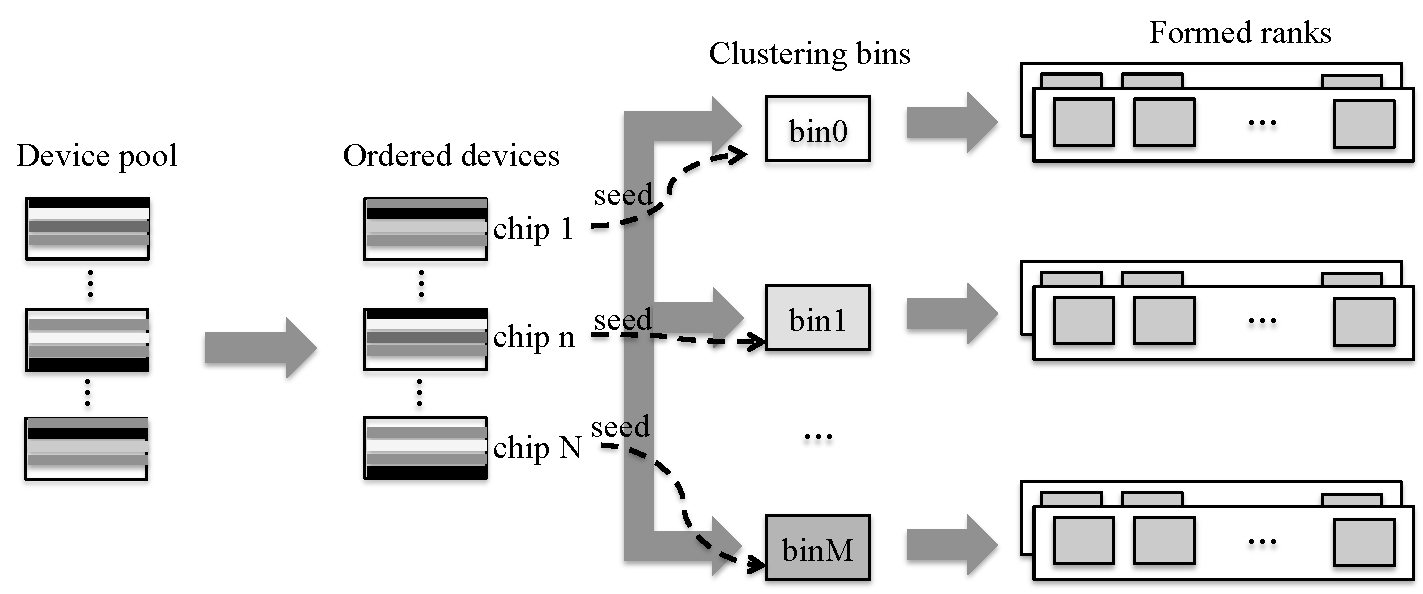
\includegraphics[width=0.8\textwidth]{figures/device_match.pdf}
\vspace{-0.15in}
\caption{Rank construction consists of three steps --- (1) chip sorting and seed chip selection;
(2) distributing chips to bins; (3) constructing DRAM ranks using chips from each bin.}
\label{fig:device_match}
  \vspace{-0.25in}
\end{figure}

We further propose to construct DRAM ranks using compatible chips, rather than random chip selection in the baseline design. 
Given $N$ DRAM chips, our goal is to construct a better rank set (and each rank contains $R$ chips). The rows in each chip are divided into $K$ chunks and we use $M$ bins to assist rank construction.

We first compute the average chip level {\tt tWR}, which uses the chunk level {\tt tWR} values of each chip. The latter can be collected during post-fabrication testing.
We sort the chips based on their average {\tt tWR} values, and choose $M$ seed chips, i.e., the chips on the sorted chip list whose indice can be divided by $\lfloor N/M\rfloor$. The seed chips are distributed to $M$ bins.

We then place the rest of chips into $M$ bins based on their similarity to the seed chip of each bin. The chunk level {\tt tWR} values of each chip are treated as a $K$-item vector. The similarity of two chips is calculated using the Hamming distance of the two $K$-item vectors. The candidate chip is placed in the bin whose seed chip has the smallest Hamming distance, i.e., the highest similarity, to the candidate chip.

Once a bin reaches its size limit, i.e., $n\times R$  where $n = \lfloor{N/M/R}\rfloor$, and $n\times R \leq N/M$, it can no longer accept new chips. In the algorithm, an extra bin $Bin_{M+1}$ is used to hold the leftover chips.
When filling chips to each bin, we construct a rank if a bin has $R$ chips (the seed chip is used to form a rank in the last batch). 

Since the algorithm needs to scan each chip and compute its similarity with all seed chips, the time complexity is $O(N\times M \times K)$. Here $M$ and $K$ are constant. $M$ is usually small ($M << N$) while $K$ can be relatively large, e.g., $K$=1024. Therefore, the time complexity is linear to the number of candidate chips. This is a light weight rank construction scheme, compared that in \cite{DAC15:radar}. Our experiments show that the two algorithms achieve similar rank level {\tt tWR} results. 
%. As a comparison, 
%the recently proposed rank construction scheme \cite{DAC15:radar} needs to sort the candidate chips continuously, which results in time complexity up to $O(N^3)$. 

\subsection{Restore Time aware Page Allocation}
\label{subsec:page_alloc}
%The translation of virtual to physical address is supported in hardware by Memory Management Unit (MMU), and the virtual-physical mapping is determined by operating system (OS). 
Traditional page allocation is restore time oblivious as all physical pages have the same access latency. However, when a set of fast DRAM chunks are constructed and exposed to the memory controller, %it is beneficial to exploit the access latency difference to speed up program execution. 
the memory system can be more effective if fast chunks are assigned to service performance-critical pages. In this paper, the page criticality is estimated using its access frequency \cite{ISCA13:charm,TC01:alloc}. Studies have shown that it is usually a small subset of pages, referred to as hot pages, that are frequently accessed in modern applications \cite{ISCA09:hot_page,ICS11:hot_page,TODAES13:hot_page}. %We adopt the offline profiling approach as in \cite{ISCA13:charm} to identify hot pages.

%\begin{figure}
 %\centering
 %   	\includegraphics[width=0.8\linewidth]{figures/TODAES_data/{page.dat}.pdf}\\
  %\vspace{-0.45in}
  %\caption{The page access distributions in SPEC CPU2006.}
  %\label{fig:page}
  %\vspace{-0.1in}
%\end{figure}


%Figure \ref{fig:page} studies the page access distribution of a set of SPEC CPU2006 applications. The figure shows that different applications have very different access behaviors: for some workloads, e.g., $459.Gem$ and $470.lbm$, accesses are evenly distributed such that the number of accumulative requests grows linearly with the number of touched pages; for some other applications, e.g., $429.mcf$ and $403.gcc$, most memory accesses come from a small subset of hot pages. The hot pages are the ones to be allocated in fast DRAM chunks. Further experimental analysis shows that the majority workloads touch less than 1/8 of the total memory space, while some benchmarks (i.e., $459.lbm$ and $429.mcf$) use up all available space.

In this paper, our goal is to illustrate that a restore time aware page allocator can take advantage of the latency difference of the DRAM chunks. For this purpose, we adopt a simple strategy that profiles program execution offline \cite{ISCA13:charm} and statically allocates hot pages to fast chunks. 
In the case if profiles are not accurate, we may need to design and enable more flexible strategies, e.g., such as the detailed behavioral synthesis \cite{TODAES11:partition} 
and data migration and compression \cite{TODAES08:bankmem}. We leave this as our future work. 

\section{Architectural Enhancements}
%In this section, we'll present the architectural implementations and also the overheads.

%\subsection{Implementation}
In order to exploit restore time variations at either chip or chunk levels, a post-fabrication testing needs to be performed to detect restore time at fine-granularity. Given that cell restore time is thermal dependent --- study showed that it becomes worse at low temperature \cite{MEM14:twr}, the manufacturer needs to record the worse timing constraints under chip's allowed working conditions. The values are organized as a table (with each entry in the table recording affected timing constraints {\tt tWR}/{\tt tRAS} of its corresponding DIMM chunk) and saved in non-volatile storage in the DIMM \cite{MICRO13:rowclone}. The memory controller loads this table at boot time and schedules memory accesses accordingly.% to maximize bandwidth and avoid conflicts. 
%As an example, two READ operations cannot be scheduled back to back to a DIMM bank if the later one accesses a fast chunk and shall compete with the preceding READ for using the data bus. 

\begin{figure}[ht] % !=overrides latex; h=here; t=top; b=bottom; p=special page for floating objects
\begin{center}
%\vspace{-0.1in}
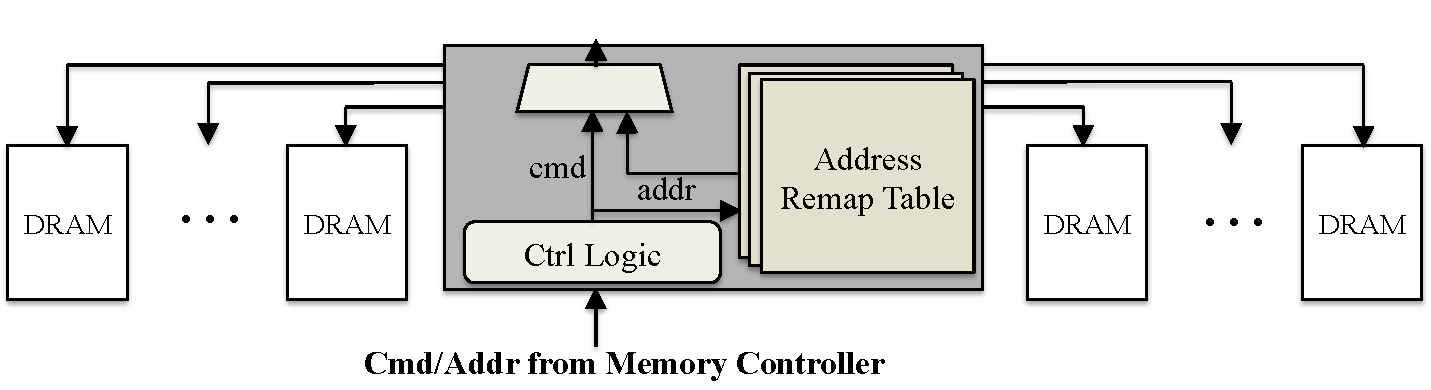
\includegraphics[width=0.7\textwidth]{figures/TODAES_data/design.pdf}
\vspace{-0.2in}
\caption{The on-DIMM architectural enhancement.}
\label{fig:design}
\end{center}
\vspace{-0.45in}
\end{figure}

To enable chunk re-organization, we need one extra chunk remapping table as shown in Figure \ref{fig:design}. Similar as HP's MC-DIMM \cite{SC09:mcdimm} and Mini-rank \cite{MICRO08:minirank}, our design integrates a bridge chip on-DIMM, which remaps the physical address sent from the memory controller to device row addresses in each chip. For the chunk remapping table, each entry maps the corresponding DIMM-chunk to the chip-chunk at each chip.  
%Given the following Table \ref{tab:art}, when the bridge chip receives a request asking for data in the 10th DIMM-chunk, it translates the requests to asking for segment data from the 1220$^{th}$ chunk from chip 0, the 124$^{th}$ chunk from chip 1, etc. 

%\begin{table}[htbp]
%\centering
%\caption{Remap table}
%\begin{tabular}{cccccccc}
%\hline
%DIMM\_chunk &chip0\_chunk &chip1\_chunk &... &chip7\_chunk \\
%\hline 
%...	 	&...	&... 	&...		&...\\
%10	 	&1220		&124 	&...		&256\\
%...	 	&...	&... 	&...		&...\\
%\hline 
%\end{tabular}
%\vspace{-0.2in}
%\label{tab:art}
%\end{table}

\section{Experimental Methodology}
\subsection{Configuration}
To evaluate the effectiveness of our designs, we compared them to traditional repair solutions using an in-house chip-multiprocessor system simulator. We modeled a quad-core system with the parameters shown in Table \ref{tab:configuration}. 

We used VARIUS to generate 90 chips, and then form ranks in different fashion discussed in Section \ref{sec:match_twr}. The memory system to be simulated is composed of two ranks. We constructed five rank pairs and tested the proposed designs with all pairs.
The DRAM timing constraints follow Hynix DDR3 SDRAM data sheet \cite{hynix:ddr3}. 
%For the schemes exploiting chunk level timing constraints, we added two CPU cycles to access the timing table.
%For the schemes performing chunk-remapping, we added one extra DRAM cycle to access the mapping table.

\begin{table}[htbp]
\vspace{-0.2in}
\centering
\caption{System Configuration}
\vspace{-0.15in}
\scalebox{0.85}
{
\begin{tabular}{l|l}
\hline\hline
Processor				&four 3.2Ghz cores; four-issue; 128 ROB size\\
\hline
				&L1(private): 64KB, 4-way, 3 cycles\\
Cache			&L2(shared): 2MB, 6-way, 32 cycles\\
				&64B cacheline\\
\hline
Memory				&Bus frequency: 1066 MHz\\
Controller 	& 128-entry queue; close page\\
\hline
			&1channel, 2ranks/channel, 8banks/rank, \\
DRAM				&16K rows/bank, 8KB/row,\\
				&1066 MHz, tCK=0.935ns, width: x8\\
\hline\hline

\end{tabular}
}
\label{tab:configuration}
\vspace{-0.2in}
\end{table}

\subsection{Workloads}
We used SPEC CPU2006 and simulated 1 billion instructions after skipping the warm-up phase of each benchmark. 
%The Read and Write MPKI (memory accesses per kilo instructions) for each workload is profiled to indicate the memory intensiveness. 
Based on MPKI, the applications are classified into three categories (Spec-High/Spec-Med/Spec-Low).%, as shown in Table \ref{tab:bench}.
The workloads are running in rate mode, where all cores execute the same task.

We performed timing simulation until all cores finish the execution, and averaged the execution time of all the four cores. We constructed five rank pairs, i.e., DIMMs. One simulation run used one DIMM while the reported results are the average of the runs using different DIMMs.

\section{Results}
We evaluated the following schemes:

--- \texttt{Baseline}. The baseline sets {\tt tWR} to 15ns, following existing specification. It is the ideal baseline due to scaling. The results of other schemes are normalized to the baseline for comparison.

--- \texttt{Relax-}$x$. Given that scaling in deep sub-micron regime leads to worse timing, this scheme relaxes time constraints to achieve x\% yield. We relaxed {\tt tWR} and set {\tt tRAS}/{\tt tRC} accordingly. We tested x=85 and x=100, respectively.

--- \texttt{Spare-}$x$. One commonly adopted post-fabrication repair approach is to integrate sparing rows/columns \cite{BOOK:jacob} to mitigate performance and yield loss. 
%It is implemented by using a laser programmable link to disconnect the abnormal rows/columns and connect the spare ones \cite{Bruce:Jacob}. 
In our experiments, we set the spare density as high as 16 spare rows per 512-row block, which resides in the aggressive spectrum \cite{BOOK:fault,SSC96:spare}. Given that spares may be reserved for high-priority repairs, such as defects and retention failures, we testsed x=0, 2, 8, 16 spares out of each 512-row block, respectively. 

--- \texttt{ECC}. ECC is implemented by placing one extra ECC chip to correct errors in data chips. Though ECC is conventionally used to correct soft errors, it can be potentially used to tolerate weak cells. Exploiting ECC chips to rescue slow rows sacrifices soft error resilience and hurts reliability \cite{DFT05:ecc}.  

--- {\tt Chunk-}$x$. This scheme implements the chunk-specific restore time control, with each bank being divided into $x$ chunks. Each DIMM chunk has its own timing constraints, which are exposed to the variation-aware memory controller.

--- \texttt{ChunkSort-}$x$. This scheme implements the chunk-specific restore time control with chunk remapping, with each bank being divided into $x$ chunks. Similar as {\tt Chunk-}$x$, the timing constraints of each chunk are exposed to the memory controller.

--- \texttt{ChunkBin-}$x$. This schemes is similar as {\tt Chunk-}$x$. The difference is that it constructs ranks using the proposed bin-based matching scheme.

--- \texttt{ChunkSortBin-}$x$.  This schemes is similar as {\tt ChunkSort-}$x$. The difference is that it constructs ranks using the proposed bin-based matching scheme.

We compared these schemes on memory access latency and system performance, and studied their sensitivity to different system configurations. 

\subsection{Execution Time}

\begin{figure}[ht]
\centering
\includegraphics[width=0.7\textwidth]{figures/TODAES_data/14nm/{stat_RAND_main-cycles.perc.dat}.pdf}
\vspace{-0.2in}
\caption{The execution time comparison of different schemes under random page allocation policy. Representative applications and the geometric means for highly memory-intensive (Spec-High) and all applications (Spec-All) are presented here.}
\label{fig:tech_time}
  \vspace{-0.25in}
\end{figure}

From Figure \ref{fig:tech_time}, we observed that 
(1) DRAM scaling has a large impact on restore time. To maintain a high yield rate, the timing constraints have to be vastly relaxed from 16 cycles to over 40 cycles, which significantly hurts performance. On average, {\tt Relax-100} and {\tt Relax-85} prolong the execution time by 37.0\% and 34.9\%, respectively. Highly memory-intensive applications tend to have large degradation (i.e., over 40\%). 
(2) Adding spare rows helps to mitigate performance losses: {\tt Spare-8} is 31.9\% worse than the ideal. 
(3) {\tt ECC} works only slightly better than {\tt Spare-8}. This is because SEC-DED ECC can only correct one bit in each 64-bit block. Since there  might be multiple cells violating timing constraints within such a 64-bit block, ECC lacks the ability to effectively adapt restore time variations.
(4) {\tt Chunk-4k} is less than 1\% better than {\tt ECC} as it exposes chunk-level restore time variations. There are a small number of chunks that have smaller tWRs than the single tWR in {\tt ECC}. Due to random page allocation policy, the exposed fast chunks cannot be fully exploited, and thus the performance improvement is pretty limited.
(5) {\tt ChunkSort-4k} works better than {\tt Chunk-4k} because it helps to construct more fast chunks. On average,
{\tt ChunkSort-4k} helps to reduce the performance loss from 37\% in {\tt Relax-100} to 26.5\%, and 4\% better than {\tt Chunk-4k} for {\tt Spec-High}.

In addition, restore time aware rank construction helps to reduce tWR ---  {\tt ChunkBin-4k} is 3\% better than  {\tt Chunk-4k} while  {\tt ChunkSortBin-4k} is 4.8\% better than  {\tt ChunkSort-4k}. 
Interestingly, {\tt ChunkBin-4k} and {\tt ChunkSort-4k} achieve comparable performance improvements over the baseline. While both schemes require post-chip-fabrication testing to extract chunk level tWR values, the former needs rank clustering, which imposes extra step and cost during fabrication; the latter needs to embed mapping table and thus introduces extra runtime overhead.  
{\tt ChunkSortBin-4k} achieves the best performance while it incurs both extra fabrication cost and runtime overhead. 

\subsection{Page Allocation Effects}

Figure \ref{fig:tech_time_14nm} compare the results using random and restore-time-aware page allocation schemes.
From the figure, by making better use of fast chunks, restore time aware page allocation speeds up the execution of all chunk based schemes, e.g., for {\tt ChunkSortBin-4k}, restore time aware allocation achieves 15\% improvement over random allocation.
Restore time aware allocation is very effective for most benchmark programs --- on average, {\tt ChunkSortBin-4k} is only 2\% worse than the ideal {\tt Baseline}. 

\begin{figure}
\centering

\begin{minipage}[b]{0.42\linewidth}
\centering
\includegraphics[width=\linewidth]{figures/TODAES_data/14nm/{RAND_small.dat}.pdf}\\
\subcaption{With random page allocation}%\label{fig:20nm_main}
\end{minipage}%
\begin{minipage}[b]{0.42\linewidth}
\centering
\includegraphics[width=\linewidth]{figures/TODAES_data/14nm/{PROF_small.dat}.pdf}\\
\subcaption{With restore time aware page allocation}%\label{fig:14nm_main}
\end{minipage}%
\vspace{-0.4in}
\caption{The execution time comparison of different schemes at 14nm technology node.}
\label{fig:tech_time_14nm}
\vspace{-0.45in}
\end{figure}


In the figure, $470.lbm$ achieves small improvement because it evenly accesses a large number of memory pages and lacks very hot pages.  Given that a small number of chunks have shorter than 15ns tWR values, it is not surprising to find that some benchmark programs, e.g., $403.gcc$ and $400.per$, have their hot pages fit in these fast chunks and thus outperform {\tt Baseline}.

Also in the figure, we observed that the effectiveness of restore time aware rank construction is diminishing after adopting restore time aware allocation. For example, on average, {\tt ChunkSort-4k} and {\tt ChunkSortBin-4k} have less than 1\% difference when using restore time aware allocation. 
Nevertheless, those benchmarks with large footprint and relatively uniform access pattern, e.g., $470.lbm$, can still achieve distinct benefits.

\subsection{Further Studies}
The effectiveness of conventional Sparing technique strongly depends on the sparing levels being used; the proposed chunk-based schemes depends on the chunk granularity. Hence, we conducted sensitivity studies on these two key parameters. 
And the experimental results show that diminishing returns using more spares because of increasingly more slow cells.
As expected, the study varying number of chunks shows that higher improvement can be achieved with increasing storage and latency overheads.

\section{Conclusion}
In this work, we studied DRAM scaling effects on restore time, and showed that future DRAM chips need relaxed timing constraints to maintain high yield and to keep the manufacturing cost low. Existing approaches are ineffective to address the performance losses. 
We proposed schemes to expose restore time variations at chunk level and devised architectural enhancements to enable find-grained variation-aware scheduling. We then proposed restore time aware rank construction and page aware page allocation schemes to make better use of fast chunks. The experimental results show that our schemes achieve as high as 25\% average performance improvement over traditional solutions.

